% ============================================================
% 讲义 — 人教版七年级上册 第4章 几何初步认识
% 编译命令：xelatex -interaction=nonstopmode 第4章_几何初步认识.tex
% ============================================================
\documentclass[12pt, a4paper]{ctexart}
\usepackage[margin=2.2cm]{geometry}
\usepackage{amsmath, amssymb}
\usepackage{enumitem}
\usepackage{tcolorbox}
\usepackage{booktabs}
\usepackage{array}
\usepackage{fancyhdr}
\usepackage{xcolor}
\usepackage{tikz}
\usepackage{hyperref}
\usepackage{graphicx}
\usepackage{multirow}
\usepackage{pgfplots}
\pgfplotsset{compat=1.18}

% 颜色定义
\definecolor{mainblue}{RGB}{41, 98, 168}
\definecolor{lightblue}{RGB}{230, 240, 255}
\definecolor{tipgreen}{RGB}{34, 139, 87}
\definecolor{lightgreen}{RGB}{235, 250, 240}
\definecolor{warnred}{RGB}{200, 50, 50}
\definecolor{lightred}{RGB}{255, 240, 240}
\definecolor{examorange}{RGB}{210, 120, 20}
\definecolor{lightorange}{RGB}{255, 248, 235}
\definecolor{apppurple}{RGB}{120, 60, 170}
\definecolor{lightpurple}{RGB}{245, 238, 255}

% 页眉页脚
\pagestyle{fancy}
\fancyhf{}
\fancyhead[L]{\small\textcolor{mainblue}{\textbf{人教版七年级上册 · 第4章 几何初步认识}}}
\fancyhead[R]{\small\textcolor{mainblue}{家教讲义}}
\fancyfoot[C]{\small —\ \thepage\ —}
\renewcommand{\headrulewidth}{0.6pt}
\renewcommand{\headrule}{\hbox to\headwidth{\color{mainblue}\leaders\hrule height \headrulewidth\hfill}}
\renewcommand{\footrulewidth}{0pt}

% tcolorbox 样式
\newtcolorbox{knowledgebox}[1][]{%
  colback=lightblue, colframe=mainblue,
  fonttitle=\bfseries\large, title=#1,
  arc=3mm, boxrule=0.8pt,
  left=8pt, right=8pt, top=6pt, bottom=6pt
}

\newtcolorbox{tipbox}[1][]{%
  colback=lightgreen, colframe=tipgreen,
  fonttitle=\bfseries, title=#1,
  arc=2mm, boxrule=0.6pt,
  left=6pt, right=6pt, top=4pt, bottom=4pt
}

\newtcolorbox{warnbox}[1][]{%
  colback=lightred, colframe=warnred,
  fonttitle=\bfseries, title=#1,
  arc=2mm, boxrule=0.6pt,
  left=6pt, right=6pt, top=4pt, bottom=4pt
}

\newtcolorbox{examplebox}[1][]{%
  colback=lightorange, colframe=examorange,
  fonttitle=\bfseries, title=#1,
  arc=3mm, boxrule=0.8pt,
  left=8pt, right=8pt, top=6pt, bottom=6pt
}

\newtcolorbox{appbox}[1][]{%
  colback=lightpurple, colframe=apppurple,
  fonttitle=\bfseries, title=#1,
  arc=3mm, boxrule=0.8pt,
  left=8pt, right=8pt, top=6pt, bottom=6pt
}

\setCJKmainfont{Hiragino Sans GB}
\setCJKsansfont{Heiti SC}

\begin{document}

% ============ 标题页 ============
\begin{center}
{\Huge\bfseries\textcolor{mainblue}{第4章\quad 几何初步认识}}\\[12pt]
{\Large\textcolor{gray}{家\quad 教\quad 讲\quad 义}}\\[8pt]
\rule{0.6\textwidth}{1pt}\\[8pt]
{\normalsize 适用：人教版\quad 七年级上册\quad |\quad 课时：6课时}
\end{center}
\vspace{10pt}

% ================================================================
% 第一部分：知识点讲解
% ================================================================
\section*{\textcolor{mainblue}{一、知识点讲解}}

% ---------- 4.1 直线、射线、线段 ----------
\subsection*{4.1\quad 直线、射线、线段}

\begin{knowledgebox}[直线]
\textbf{直线}没有端点，可以向两端无限延伸，无法度量长度。

\textbf{表示方法：}
\begin{itemize}[nosep]
  \item 用直线上两个点的大写字母表示，如直线 $AB$（或直线 $BA$）；
  \item 用一个小写字母表示，如直线 $l$。
\end{itemize}

\begin{center}
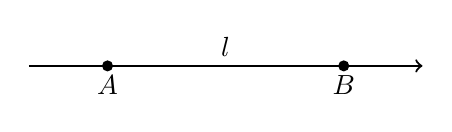
\begin{tikzpicture}
  \draw[thick, ->] (-2,0) -- (3,0);
  \fill (-1,0) circle (2pt) node[below] {$A$};
  \fill (2,0) circle (2pt) node[below] {$B$};
  \node[above] at (0.5,0) {$l$};
\end{tikzpicture}
\end{center}
\end{knowledgebox}

\begin{knowledgebox}[射线]
\textbf{射线}有一个端点，只能向一个方向无限延伸，无法度量长度。

\textbf{表示方法：}用端点和射线上另一个点的大写字母表示，\textbf{端点字母写在前面}。如射线 $OA$（$O$ 为端点）。

\begin{center}
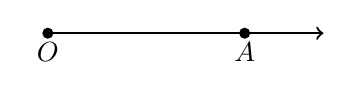
\begin{tikzpicture}
  \fill (0,0) circle (2pt) node[below] {$O$};
  \draw[thick, ->] (0,0) -- (3.5,0);
  \fill (2.5,0) circle (2pt) node[below] {$A$};
\end{tikzpicture}
\end{center}
\end{knowledgebox}

\begin{knowledgebox}[线段]
\textbf{线段}有两个端点，不能延伸，\textbf{可以度量长度}。

\textbf{表示方法：}用两个端点的大写字母表示，如线段 $AB$（或线段 $BA$）；也可用一个小写字母表示，如线段 $a$。

\begin{center}
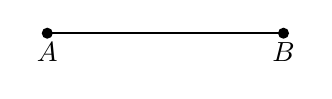
\begin{tikzpicture}
  \fill (0,0) circle (2pt) node[below] {$A$};
  \fill (3,0) circle (2pt) node[below] {$B$};
  \draw[thick] (0,0) -- (3,0);
\end{tikzpicture}
\end{center}
\end{knowledgebox}

\begin{warnbox}[直线、射线、线段的区别]
\begin{center}
\renewcommand{\arraystretch}{1.3}
\begin{tabular}{|c|c|c|c|}
\hline
 & \textbf{端点数} & \textbf{能否延伸} & \textbf{能否度量} \\
\hline
直线 & 0个 & 向两端无限延伸 & 不能 \\
\hline
射线 & 1个 & 向一端无限延伸 & 不能 \\
\hline
线段 & 2个 & 不能延伸 & 能 \\
\hline
\end{tabular}
\end{center}
\textbf{注意：}射线 $AB$ 和射线 $BA$ 是不同的射线（端点不同）！但线段 $AB$ 和线段 $BA$ 是同一条线段。
\end{warnbox}

% ---------- 4.2 直线的性质 ----------
\subsection*{4.2\quad 直线的性质}

\begin{knowledgebox}[两点确定一条直线]
\textbf{基本事实：}经过两点\textbf{有且只有}一条直线。

简单说就是：\textbf{两点确定一条直线}。

这条性质说明：
\begin{itemize}[nosep]
  \item \textbf{存在性}：经过两点一定有一条直线；
  \item \textbf{唯一性}：经过两点只有一条直线，不会有第二条。
\end{itemize}

\textbf{生活应用：}植树时先确定两棵树的位置，就能拉出一条直线；砌墙时用两点确定一条线来对齐。
\end{knowledgebox}

\begin{knowledgebox}[两点之间线段最短]
\textbf{基本事实：}两点之间，\textbf{线段最短}。

即连接两点的所有线（曲线、折线等）中，线段的长度是最短的。

两点之间线段的长度，叫做这两点之间的\textbf{距离}。
\end{knowledgebox}

% ---------- 4.3 线段的中点与和差 ----------
\subsection*{4.3\quad 线段的中点与和差}

\begin{knowledgebox}[线段的中点]
把一条线段分成\textbf{两条相等的线段}的点，叫做这条线段的\textbf{中点}。

如图，若 $M$ 是线段 $AB$ 的中点，则：
$$AM=MB=\frac{1}{2}AB$$

\begin{center}
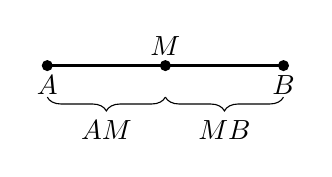
\begin{tikzpicture}
  \fill (0,0) circle (2pt) node[below] {$A$};
  \fill (3,0) circle (2pt) node[below] {$B$};
  \fill (1.5,0) circle (2pt) node[above] {$M$};
  \draw[thick] (0,0) -- (3,0);
  \draw[decorate, decoration={brace, mirror, amplitude=5pt}] (0,-0.4) -- (1.5,-0.4) node[midway, below=5pt] {$AM$};
  \draw[decorate, decoration={brace, mirror, amplitude=5pt}] (1.5,-0.4) -- (3,-0.4) node[midway, below=5pt] {$MB$};
\end{tikzpicture}
\end{center}
\end{knowledgebox}

\begin{knowledgebox}[线段的和与差]
两条线段可以进行加法和减法运算。

如图，设线段 $AB=a$，线段 $BC=b$，且点 $B$ 在线段 $AC$ 上：

\begin{center}
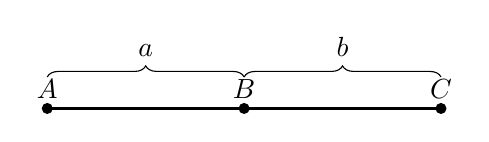
\begin{tikzpicture}
  \fill (0,0) circle (2pt) node[above] {$A$};
  \fill (2.5,0) circle (2pt) node[above] {$B$};
  \fill (5,0) circle (2pt) node[above] {$C$};
  \draw[thick] (0,0) -- (5,0);
  \draw[decorate, decoration={brace, amplitude=4pt}] (0,0.4) -- (2.5,0.4) node[midway, above=4pt] {$a$};
  \draw[decorate, decoration={brace, amplitude=4pt}] (2.5,0.4) -- (5,0.4) node[midway, above=4pt] {$b$};
\end{tikzpicture}
\end{center}

则 $AC=AB+BC=a+b$。

反之，$AB=AC-BC$，$BC=AC-AB$。
\end{knowledgebox}

% ---------- 4.4 角的概念和表示 ----------
\subsection*{4.4\quad 角的概念和表示}

\begin{knowledgebox}[角的概念]
\textbf{角}是由两条具有\textbf{公共端点}的\textbf{射线}组成的图形。这个公共端点叫做角的\textbf{顶点}，两条射线叫做角的\textbf{两条边}。

角也可以看作一条射线绕着它的端点从一个位置旋转到另一个位置所形成的图形。

\begin{center}
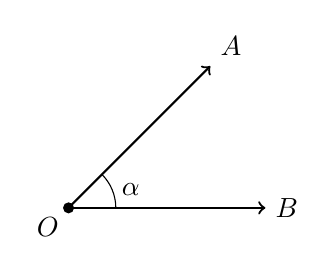
\begin{tikzpicture}
  \fill (0,0) circle (2pt) node[below left] {$O$};
  \draw[thick, ->] (0,0) -- (2.5,0) node[right] {$B$};
  \draw[thick, ->] (0,0) -- (1.8,1.8) node[above right] {$A$};
  \draw (0.6,0) arc (0:45:0.6) node[midway, right] {$\alpha$};
\end{tikzpicture}
\end{center}
\end{knowledgebox}

\begin{knowledgebox}[角的表示方法]
角有以下三种表示方法：
\begin{enumerate}[nosep]
  \item 用三个大写字母表示，顶点字母写在中间，如 $\angle AOB$（或 $\angle BOA$）；
  \item 用一个大写字母表示（顶点处只有一个角时），如 $\angle O$；
  \item 用一个数字或希腊字母标注，如 $\angle 1$、$\angle\alpha$。
\end{enumerate}

\textbf{注意：}用一个大写字母表示时，顶点处必须只有一个角，否则会产生歧义。
\end{knowledgebox}

\begin{knowledgebox}[角的度量单位及换算]
角的度量单位是\textbf{度}（$^\circ$）、\textbf{分}（$'$）、\textbf{秒}（$''$）。

换算关系：
$$1^\circ=60',\quad 1'=60'',\quad 1^\circ=3600''$$

\textbf{角的分类：}
\begin{itemize}[nosep]
  \item 锐角：$0^\circ<\alpha<90^\circ$
  \item 直角：$\alpha=90^\circ$
  \item 钝角：$90^\circ<\alpha<180^\circ$
  \item 平角：$\alpha=180^\circ$
  \item 周角：$\alpha=360^\circ$
\end{itemize}
\end{knowledgebox}

\begin{warnbox}[度分秒换算易错点]
\begin{itemize}[nosep]
  \item 度分秒之间的进率是\textbf{60}（不是100！），和时间的时分秒类似。
  \item 大单位化小单位要\textbf{乘}60，小单位化大单位要\textbf{除以}60。
  \item 计算时注意：$2.5^\circ\neq 2^\circ50'$，正确为 $2.5^\circ=2^\circ30'$。
\end{itemize}
\end{warnbox}

% ---------- 4.5 角的和差 ----------
\subsection*{4.5\quad 角的和差}

\begin{knowledgebox}[角的和与差]
两个角可以进行加法和减法运算。

如果 $\angle AOB=\alpha$，$\angle BOC=\beta$，且射线 $OB$ 在 $\angle AOC$ 的内部，则：

$$\angle AOC=\angle AOB+\angle BOC=\alpha+\beta$$

\begin{center}
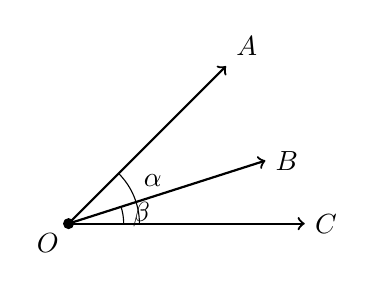
\begin{tikzpicture}
  \fill (0,0) circle (2pt) node[below left] {$O$};
  \draw[thick, ->] (0,0) -- (3,0) node[right] {$C$};
  \draw[thick, ->] (0,0) -- (2,2) node[above right] {$A$};
  \draw[thick, ->] (0,0) -- (2.5,0.8) node[right] {$B$};
  \draw (0.7,0) arc (0:18:0.7) node[midway, right] {$\beta$};
  \draw (0.9,0) arc (0:45:0.9) node[midway, above right] {$\alpha$};
\end{tikzpicture}
\end{center}

反之：$\angle AOB=\angle AOC-\angle BOC$，$\angle BOC=\angle AOC-\angle AOB$。
\end{knowledgebox}

% ---------- 4.6 角的平分线 ----------
\subsection*{4.6\quad 角的平分线}

\begin{knowledgebox}[角的平分线]
从一个角的顶点出发，把这个角分成\textbf{两个相等的角}的射线，叫做这个角的\textbf{平分线}。

如图，若射线 $OC$ 是 $\angle AOB$ 的平分线，则：
$$\angle AOC=\angle COB=\frac{1}{2}\angle AOB$$

\begin{center}
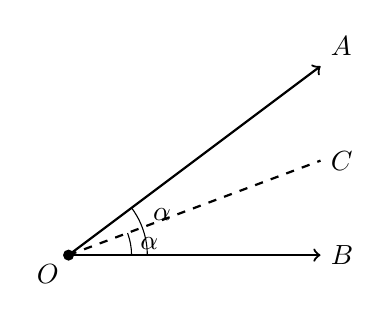
\begin{tikzpicture}
  \fill (0,0) circle (2pt) node[below left] {$O$};
  \draw[thick, ->] (0,0) -- (3.2,0) node[right] {$B$};
  \draw[thick, ->] (0,0) -- (3.2,2.4) node[above right] {$A$};
  \draw[thick, dashed] (0,0) -- (3.2,1.2) node[right] {$C$};
  \draw (0.8,0) arc (0:20.5:0.8) node[midway, right] {$\alpha$};
  \draw (1,0) arc (0:36.87:1) node[midway, above right] {$\alpha$};
\end{tikzpicture}
\end{center}
\end{knowledgebox}

% ---------- 4.7 余角和补角 ----------
\subsection*{4.7\quad 余角和补角}

\begin{knowledgebox}[互余与互补]
\textbf{互余（互为余角）：}如果两个角的和等于 $90^\circ$（直角），那么这两个角互为余角，简称\textbf{互余}。

即若 $\angle\alpha+\angle\beta=90^\circ$，则 $\angle\alpha$ 与 $\angle\beta$ 互余。

\textbf{互补（互为补角）：}如果两个角的和等于 $180^\circ$（平角），那么这两个角互为补角，简称\textbf{互补}。

即若 $\angle\alpha+\angle\beta=180^\circ$，则 $\angle\alpha$ 与 $\angle\beta$ 互补。
\end{knowledgebox}

\begin{knowledgebox}[余角和补角的性质]
\textbf{性质1：}同角（等角）的余角相等。

\begin{itemize}[nosep]
  \item 若 $\angle\alpha+\angle\beta=90^\circ$，$\angle\alpha+\angle\gamma=90^\circ$，则 $\angle\beta=\angle\gamma$。
  \item 若 $\angle\alpha=\angle\alpha'$，$\angle\alpha+\angle\beta=90^\circ$，$\angle\alpha'+\angle\gamma=90^\circ$，则 $\angle\beta=\angle\gamma$。
\end{itemize}

\textbf{性质2：}同角（等角）的补角相等。

\begin{itemize}[nosep]
  \item 若 $\angle\alpha+\angle\beta=180^\circ$，$\angle\alpha+\angle\gamma=180^\circ$，则 $\angle\beta=\angle\gamma$。
\end{itemize}
\end{knowledgebox}

\begin{tipbox}[记忆技巧]
\begin{itemize}[nosep]
  \item \textbf{余角}：和为 $90^\circ$，"余"谐音"鱼"，鱼在水里，水温约 $90^\circ$（想象记忆）。
  \item \textbf{补角}：和为 $180^\circ$，"补"谐音"布"，布展开是平角 $180^\circ$。
  \item 互余、互补只看\textbf{角度之和}，与两个角的位置是否相邻\textbf{无关}。
  \item 锐角才有余角；大于 $0^\circ$ 且小于 $180^\circ$ 的角才有补角。
\end{itemize}
\end{tipbox}

% ---------- 4.8 方位角 ----------
\subsection*{4.8\quad 方位角}

\begin{knowledgebox}[方位角]
\textbf{方位角}是以正北或正南方向为基准，描述目标方向的角度。

表示规则：
\begin{itemize}[nosep]
  \item 先说"北偏东""北偏西""南偏东""南偏西"；
  \item 再说偏转的角度。
\end{itemize}

例如："北偏东 $30^\circ$"表示从正北方向顺时针偏转 $30^\circ$。

\begin{center}
\begin{tikzpicture}
  \draw[thick, ->] (0,-0.3) -- (0,3) node[above] {\small 北};
  \draw[thick, ->] (0,-0.3) -- (3,-0.3) node[right] {\small 东};
  \draw[thick, ->] (0,-0.3) -- (-3,-0.3) node[left] {\small 西};
  \draw[thick, ->] (0,-0.3) -- (0,-3) node[below] {\small 南};
  \draw[thick, blue, ->] (0,0) -- (2.2,1.27) node[right, blue] {\small 北偏东$30^\circ$};
  \draw (0,1.5) arc (90:60:1.5) node[midway, left] {\small $30^\circ$};
  \draw[thick, red, ->] (0,0) -- (-1.8,1.04) node[left, red] {\small 北偏西$30^\circ$};
  \draw (0,1.2) arc (90:120:1.2) node[midway, right] {\small $30^\circ$};
\end{tikzpicture}
\end{center}

\textbf{注意：}方位角总是以"北"或"南"为基准，不能说"东偏北"。
\end{knowledgebox}

% ================================================================
% 第二部分：例题精讲
% ================================================================
\section*{\textcolor{examorange}{二、例题精讲}}

\begin{examplebox}[【例题1】基础：线段中点的计算]
如图，已知线段 $AB=12\text{ cm}$，$C$ 是 $AB$ 的中点，$D$ 是 $CB$ 的中点。求 $CD$ 的长度。

\begin{center}
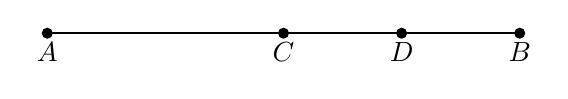
\begin{tikzpicture}
  \fill (0,0) circle (2pt) node[below] {$A$};
  \fill (3,0) circle (2pt) node[below] {$C$};
  \fill (4.5,0) circle (2pt) node[below] {$D$};
  \fill (6,0) circle (2pt) node[below] {$B$};
  \draw[thick] (0,0) -- (6,0);
\end{tikzpicture}
\end{center}
\end{examplebox}

\textbf{解：}

因为 $C$ 是 $AB$ 的中点，所以：
$$AC=CB=\frac{1}{2}AB=\frac{1}{2}\times 12=6\text{ cm}$$

因为 $D$ 是 $CB$ 的中点，所以：
$$CD=\frac{1}{2}CB=\frac{1}{2}\times 6=3\text{ cm}$$

\textbf{答：}$CD$ 的长度为 $3\text{ cm}$。

\vspace{6pt}

\begin{examplebox}[【例题2】基础：角度计算]
计算下列各题：
\begin{enumerate}[nosep]
  \item $45^\circ36'+28^\circ45'=$ ？
  \item $90^\circ-56^\circ23'=$ ？
  \item $25^\circ24'=$ ？$^\circ$
\end{enumerate}
\end{examplebox}

\textbf{解：}

(1) $45^\circ36'+28^\circ45'$

$=45^\circ+28^\circ+36'+45'$

$=73^\circ+81'$

$=73^\circ+1^\circ21'$

$=74^\circ21'$

\medskip

(2) $90^\circ-56^\circ23'$

$=89^\circ60'-56^\circ23'$

$=33^\circ37'$

\medskip

(3) $25^\circ24'$

$=25^\circ+\dfrac{24'}{60}=25^\circ+0.4^\circ=25.4^\circ$

\begin{warnbox}[易错提醒]
$25^\circ24'$ 不等于 $25.24^\circ$！因为分和度之间的进率是60，不是100。正确计算为 $24\div 60=0.4$，所以 $25^\circ24'=25.4^\circ$。
\end{warnbox}

\vspace{6pt}

\begin{examplebox}[【例题3】易错：射线与角的概念辨析]
下列说法正确的是（\quad）
\begin{enumerate}[label=\Alph*., nosep]
  \item 射线 $OA$ 和射线 $AO$ 是同一条射线
  \item 直线比射线长
  \item 线段 $AB$ 和线段 $BA$ 是同一条线段
  \item 平角就是一条直线
\end{enumerate}
\end{examplebox}

\textbf{解：}

\textbf{选C。}

分析各选项：

A. 射线 $OA$ 的端点是 $O$，射线 $AO$ 的端点是 $A$，端点不同，\textbf{不是}同一条射线。错误。

B. 直线和射线都是无限延伸的，无法度量长度，不能比较"谁更长"。错误。

C. 线段 $AB$ 和线段 $BA$ 的端点相同，只是表示顺序不同，是\textbf{同一条线段}。正确。

D. 平角的两条边在同一条直线上，但平角有顶点和两条边的概念，和"一条直线"是不同的。错误。

\vspace{6pt}

\begin{examplebox}[【例题4】综合：角平分线与角度计算]
如图，已知 $\angle AOB=80^\circ$，$OC$ 是 $\angle AOB$ 的平分线，$OD$ 是 $\angle COB$ 的平分线。求 $\angle AOD$ 的度数。

\begin{center}
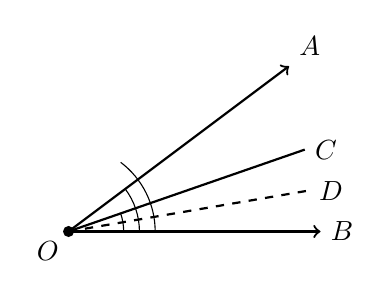
\begin{tikzpicture}
  \fill (0,0) circle (2pt) node[below left] {$O$};
  \draw[thick, ->] (0,0) -- (3.2,0) node[right] {$B$};
  \draw[thick, ->] (0,0) -- (2.8,2.1) node[above right] {$A$};
  \draw[thick] (0,0) -- (3,1.04) node[right] {$C$};
  \draw[thick, dashed] (0,0) -- (3.05,0.52) node[right] {$D$};
  \draw (0.7,0) arc (0:19:0.7);
  \draw (0.9,0) arc (0:37:0.9);
  \draw (1.1,0) arc (0:53:1.1);
\end{tikzpicture}
\end{center}
\end{examplebox}

\textbf{解：}

因为 $OC$ 是 $\angle AOB$ 的平分线，所以：
$$\angle BOC=\frac{1}{2}\angle AOB=\frac{1}{2}\times 80^\circ=40^\circ$$

因为 $OD$ 是 $\angle COB$ 的平分线，所以：
$$\angle BOD=\frac{1}{2}\angle BOC=\frac{1}{2}\times 40^\circ=20^\circ$$

因此：
$$\angle AOD=\angle AOB-\angle BOD=80^\circ-20^\circ=60^\circ$$

\textbf{答：}$\angle AOD=60^\circ$。

\vspace{6pt}

\begin{examplebox}[【例题5】综合：互余与互补的应用]
已知 $\angle\alpha$ 与 $\angle\beta$ 互补，且 $\angle\alpha-\angle\beta=30^\circ$。求 $\angle\alpha$ 和 $\angle\beta$ 的度数。
\end{examplebox}

\textbf{解：}

根据题意，列方程组：
$$\begin{cases} \angle\alpha+\angle\beta=180^\circ \\ \angle\alpha-\angle\beta=30^\circ \end{cases}$$

两式相加：$2\angle\alpha=210^\circ$，所以 $\angle\alpha=105^\circ$。

代入第一个式子：$105^\circ+\angle\beta=180^\circ$，所以 $\angle\beta=75^\circ$。

\textbf{答：}$\angle\alpha=105^\circ$，$\angle\beta=75^\circ$。

\textbf{检验：}$105^\circ+75^\circ=180^\circ$（互补）$\checkmark$，$105^\circ-75^\circ=30^\circ$ $\checkmark$。

\vspace{6pt}

\begin{examplebox}[【例题6】综合提高：线段和差的证明]
如图，$C$ 是线段 $AB$ 上一点，$M$ 是 $AC$ 的中点，$N$ 是 $CB$ 的中点。求证：$MN=\dfrac{1}{2}AB$。

\begin{center}
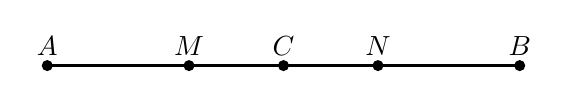
\begin{tikzpicture}
  \fill (0,0) circle (2pt) node[above] {$A$};
  \fill (1.8,0) circle (2pt) node[above] {$M$};
  \fill (3,0) circle (2pt) node[above] {$C$};
  \fill (4.2,0) circle (2pt) node[above] {$N$};
  \fill (6,0) circle (2pt) node[above] {$B$};
  \draw[thick] (0,0) -- (6,0);
\end{tikzpicture}
\end{center}
\end{examplebox}

\textbf{证明：}

因为 $M$ 是 $AC$ 的中点，所以 $MC=\dfrac{1}{2}AC$。

因为 $N$ 是 $CB$ 的中点，所以 $CN=\dfrac{1}{2}CB$。

又因为 $MN=MC+CN$，所以：

$$MN=\frac{1}{2}AC+\frac{1}{2}CB=\frac{1}{2}(AC+CB)$$

因为 $AC+CB=AB$，所以：

$$MN=\frac{1}{2}AB$$

证毕。$\blacksquare$

\vspace{6pt}

\begin{examplebox}[【例题7】方位角的应用]
如图，从点 $O$ 观测，点 $A$ 在北偏东 $40^\circ$ 方向，点 $B$ 在南偏东 $25^\circ$ 方向。求 $\angle AOB$ 的度数。

\begin{center}
\begin{tikzpicture}
  \fill (0,0) circle (2pt) node[below] {$O$};
  \draw[thick, ->] (0,-0.2) -- (0,3) node[above] {\small 北};
  \draw[thick, ->] (0,-0.2) -- (0,-3) node[below] {\small 南};
  \draw[thick, blue, ->] (0,0) -- (2,2.4) node[above right] {$A$};
  \draw[thick, red, ->] (0,0) -- (1.7,-2.6) node[below right] {$B$};
  \draw (0,1.5) arc (90:50:1.5) node[midway, right] {\small $40^\circ$};
  \draw (0,-1.2) arc (270:245:1.2) node[midway, right] {\small $25^\circ$};
\end{tikzpicture}
\end{center}
\end{examplebox}

\textbf{解：}

$\angle AOB$ 可以分解为：$\angle AOB=\angle AON+\angle NOB$

其中 $ON$ 为正南方向（与正北方向相反），$\angle NOB=25^\circ$。

正北和正南方向之间的夹角为 $180^\circ$，所以：

$\angle AON=180^\circ-40^\circ=140^\circ$（$A$ 在北偏东 $40^\circ$，从正南方向到 $A$ 的角度）

等等，让我重新分析。

从正北方向顺时针到 $OA$ 为 $40^\circ$，从正南方向逆时针到 $OB$ 为 $25^\circ$（即南偏东 $25^\circ$）。

正北到正南为 $180^\circ$，所以从正北顺时针到 $OB$ 的角度为 $180^\circ-25^\circ=155^\circ$。

$$\angle AOB=155^\circ-40^\circ=115^\circ$$

\textbf{答：}$\angle AOB=115^\circ$。

% ================================================================
% 第三部分：应用题
% ================================================================
\section*{\textcolor{apppurple}{三、应用题}}

\begin{appbox}[【应用1】时钟角度问题]
在 $3$ 点整时，钟面上时针和分针所成的角是多少度？这个角是什么角（锐角/直角/钝角）？
\end{appbox}

\textbf{解：}

钟面一圈为 $360^\circ$，共有 $12$ 个大格，每个大格对应 $360^\circ\div 12=30^\circ$。

$3$ 点整时，分针指向 $12$，时针指向 $3$，两针之间有 $3$ 个大格。

所以两针所成的角 $=3\times 30^\circ=90^\circ$。

\textbf{答：}$3$ 点整时时针和分针所成的角为 $90^\circ$，这是一个直角。

\begin{center}
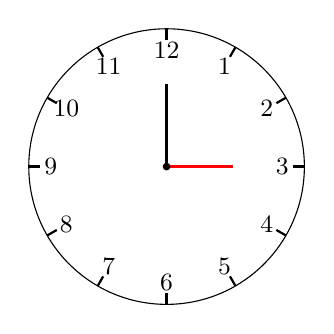
\begin{tikzpicture}[scale=0.7]
  \draw (0,0) circle (2.5);
  \foreach \i in {1,...,12}{
    \pgfmathsetmacro{\angle}{90-\i*30}
    \node at (\angle:2.1) {\small \i};
    \draw[thick] (\angle:2.3) -- (\angle:2.5);
  }
  \draw[thick] (0,0) -- (90:1.5);  % 分针指向12
  \draw[thick, red] (0,0) -- (0:1.2);  % 时针指向3
  \fill (0,0) circle (2pt);
\end{tikzpicture}
\end{center}

\vspace{6pt}

\begin{appbox}[【应用2】方位角问题——航行路线]
一艘船从港口 $O$ 出发，先向北偏东 $50^\circ$ 方向航行了 $20$ 海里到达 $A$ 处，然后从 $A$ 处改变航向，向南偏东 $30^\circ$ 方向继续航行。求在 $A$ 处转弯时航向改变的角度（即 $\angle OAB$ 的补角 $-\angle$外角）。
\end{appbox}

\textbf{解：}

先画示意图分析。设正北方向为 $ON$。

\begin{center}
\begin{tikzpicture}[scale=0.8]
  \fill (0,0) circle (2pt) node[below left] {$O$};
  \fill (3,2) circle (2pt) node[above right] {$A$};
  \fill (0,3.5) node[above] {\small 北};
  \draw[thick, ->] (0,0) -- (0,3.2);
  \draw[thick, blue, ->] (0,0) -- (3.2,2.2) node[midway, above left] {\small $20$海里};
  \draw[thick, red, ->] (3,2) -- (5.5,0.7) node[right] {$B$};
  % 角度标注
  \draw (0,1.2) arc (90:55:1.2) node[midway, right] {\small $50^\circ$};
  \draw[dashed] (3,2) -- (3,4);
  \draw (3,3) arc (90:120:1) node[midway, left] {\small $30^\circ$};
\end{tikzpicture}
\end{center}

从 $A$ 处出发的航向为南偏东 $30^\circ$。我们需要求在 $A$ 处的转向角度。

在 $A$ 点处，$OA$ 的延长线方向（从 $O$ 到 $A$ 继续前进的方向）与 $OA$ 的反向形成平角。

$OA$ 的方向是北偏东 $50^\circ$，所以 $AO$（从 $A$ 指向 $O$）的方向是南偏西 $50^\circ$。

$AB$ 的方向是南偏东 $30^\circ$。

从 $AO$ 方向（南偏西 $50^\circ$）到 $AB$ 方向（南偏东 $30^\circ$）的夹角 $=50^\circ+30^\circ=80^\circ$。

所以在 $A$ 处转向的角度为 $\angle OAB=180^\circ-80^\circ=100^\circ$（转向的角度是外角）。

\textbf{答：}船在 $A$ 处的转向角度为 $100^\circ$。

\vspace{6pt}

\begin{appbox}[【应用3】测量中的几何应用]
小明要测量学校操场上 $A$、$B$ 两点之间的距离，但中间有一堵墙无法直接测量。他先找了一个能同时看到 $A$ 和 $B$ 的点 $C$，测得 $CA=15$ 米，$CB=20$ 米。然后在 $CA$ 的延长线上找到点 $D$，使 $CD=15$ 米；在 $CB$ 的延长线上找到点 $E$，使 $CE=20$ 米。测得 $DE=25$ 米。求 $AB$ 的距离。
\end{appbox}

\textbf{解：}

由于 $D$ 在 $CA$ 延长线上且 $CD=CA=15$，所以 $C$ 是 $DA$ 的中点，即 $DA=30$ 米。

不对，$D$ 在 $CA$ 的延长线上，$CD=15$，$CA=15$，说明 $A$ 在 $CD$ 之间，且 $CA=AD$？不对。

让我重新分析：$D$ 在 $CA$ 的延长线上，即 $C$ 在 $A$ 和 $D$ 之间，$CD=15$ 米，$CA=15$ 米，所以 $A$ 和 $D$ 关于 $C$ 对称，$AD=30$ 米。不对，$D$ 在 $CA$ 的延长线上，意味着 $A$、$C$、$D$ 三点共线，且 $C$ 在 $A$、$D$ 之间？不对，"在 $CA$ 的延长线上"意味着 $D$ 在 $A$ 的另一侧，即 $A$、$C$、$D$ 共线，$A$ 在 $C$ 和 $D$ 之间。

$CA=15$，$CD=15$，$D$ 在 $CA$ 的延长线上（从 $C$ 经 $A$ 延伸），所以 $D$ 和 $A$ 重合？这不合理。

换一种理解：$D$ 在 $AC$ 的延长线上（从 $A$ 经 $C$ 延伸），即 $A$、$C$、$D$ 共线，$C$ 在 $A$、$D$ 之间。$AC=15$，$CD=15$，则 $AD=AC+CD=30$。

同理，$E$ 在 $BC$ 的延长线上，$BC=20$，$CE=20$，$BE=40$。

在 $\triangle DCE$ 和 $\triangle ACB$ 中：

$CD=CA=15$，$CE=CB=20$，$\angle DCE=\angle ACB$（对顶角）

所以 $\triangle DCE\cong\triangle ACB$（SAS），故 $AB=DE=25$ 米。

\textbf{答：}$A$、$B$ 之间的距离为 $25$ 米。

\begin{center}
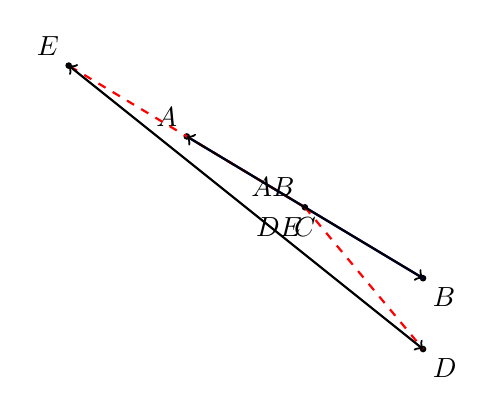
\begin{tikzpicture}[scale=0.6]
  \fill (0,0) circle (2pt) node[below] {$C$};
  \fill (-2.5,1.5) circle (2pt) node[above left] {$A$};
  \fill (2.5,-1.5) circle (2pt) node[below right] {$B$};
  \fill (2.5,-3) circle (2pt) node[below right] {$D$};
  \fill (-5,3) circle (2pt) node[above left] {$E$};
  \draw[thick, blue] (-2.5,1.5) -- (0,0) -- (2.5,-1.5);
  \draw[thick, red, dashed] (0,0) -- (2.5,-3);
  \draw[thick, red, dashed] (0,0) -- (-5,3);
  \draw[thick, <->] (-2.5,1.5) -- (2.5,-1.5) node[midway, above left] {$AB$};
  \draw[thick, <->] (-5,3) -- (2.5,-3) node[midway, below right] {$DE$};
\end{tikzpicture}
\end{center}

% ================================================================
% 第四部分：课堂练习
% ================================================================
\section*{\textcolor{tipgreen}{四、课堂练习}}

\begin{enumerate}
  \item 已知线段 $AB=8\text{ cm}$，延长 $AB$ 到 $C$，使 $BC=3\text{ cm}$。$M$ 是 $AC$ 的中点，求 $BM$ 的长度。

  \item 计算：(1) $108^\circ18'-56^\circ42'=$ ？\quad (2) $15^\circ24'\times 3=$ ？

  \item 已知 $\angle\alpha$ 的余角是 $35^\circ$，求 $\angle\alpha$ 的补角。

  \item 如图，$O$ 是直线 $AB$ 上一点，$OC$ 是从 $O$ 出发的射线，$OD$ 是 $\angle AOC$ 的平分线，$OE$ 是 $\angle BOC$ 的平分线。求 $\angle DOE$ 的度数。

\begin{center}
\begin{tikzpicture}
  \draw[thick, <->] (-3.5,0) -- (3.5,0);
  \fill (-3,0) circle (2pt) node[below] {$A$};
  \fill (0,0) circle (2pt) node[below] {$O$};
  \fill (3,0) circle (2pt) node[below] {$B$};
  \draw[thick] (0,0) -- (1.5,2.5) node[above] {$C$};
  \draw[thick, dashed] (0,0) -- (-2,1.5) node[above left] {$D$};
  \draw[thick, dashed] (0,0) -- (2.2,1.2) node[above right] {$E$};
\end{tikzpicture}
\end{center}

  \item 一个人从 $A$ 点出发，先向北偏西 $40^\circ$ 方向走了 $100$ 米到达 $B$ 点，再向南偏西 $50^\circ$ 方向走了 $100$ 米到达 $C$ 点。求 $\angle ABC$ 的度数。
\end{enumerate}

\vspace{10pt}

\begin{knowledgebox}[参考答案]
\textbf{第1题：}

$AC=AB+BC=8+3=11\text{ cm}$。$M$ 是 $AC$ 的中点，$AM=MC=\dfrac{11}{2}=5.5\text{ cm}$。

$BM=AB-AM=8-5.5=2.5\text{ cm}$。

\textbf{答：}$BM=2.5\text{ cm}$。

\medskip

\textbf{第2题：}

(1) $108^\circ18'-56^\circ42'=107^\circ78'-56^\circ42'=51^\circ36'$

(2) $15^\circ24'\times 3=45^\circ72'=46^\circ12'$

\medskip

\textbf{第3题：}

$\angle\alpha=90^\circ-35^\circ=55^\circ$

$\angle\alpha$ 的补角 $=180^\circ-55^\circ=125^\circ$

\textbf{答：}$\angle\alpha$ 的补角为 $125^\circ$。

\medskip

\textbf{第4题：}

因为 $OD$ 平分 $\angle AOC$，$OE$ 平分 $\angle BOC$，所以：

$\angle DOC=\dfrac{1}{2}\angle AOC$，$\angle COE=\dfrac{1}{2}\angle BOC$。

$\angle DOE=\angle DOC+\angle COE=\dfrac{1}{2}\angle AOC+\dfrac{1}{2}\angle BOC=\dfrac{1}{2}(\angle AOC+\angle BOC)$

因为 $A$、$O$、$B$ 共线，所以 $\angle AOC+\angle BOC=180^\circ$。

$$\angle DOE=\frac{1}{2}\times 180^\circ=90^\circ$$

\textbf{答：}$\angle DOE=90^\circ$（始终为直角，与 $OC$ 的位置无关）。

\medskip

\textbf{第5题：}

$AB$ 方向为北偏西 $40^\circ$，$BA$（反方向）为南偏东 $40^\circ$。

$BC$ 方向为南偏西 $50^\circ$。

$\angle ABC$ 是从 $BA$ 方向转到 $BC$ 方向的角度。

$BA$ 为南偏东 $40^\circ$，$BC$ 为南偏西 $50^\circ$，两方向分别在正南的两侧。

$\angle ABC=40^\circ+50^\circ=90^\circ$

\textbf{答：}$\angle ABC=90^\circ$。
\end{knowledgebox}

\vfill
\begin{center}
\small\textcolor{gray}{本讲义仅供教学参考，例题可根据学生水平调整难度。}
\end{center}

\end{document}
